\section{Generalist Robot Policies}
\label{sec:learning-foundation}

\epigraph{\textit{Specialization is for insects}}{Robert A. Heinlein}

\begin{tldr}
Openly available, large-scale datasets and the development of stable-to-train, expressive and efficient architectures fostered research on the development of generalist robot policies that can operate across embodiment and tasks.
\end{tldr}

The advent of large models trained on internet-scale datasets has drastically influenced fields like Computer Vision (CV) and Natural Language Processing (NLP), shifting the previously task-specific paradigm towards combining (1) an initial, task-agnostic large-scale pre-training stage and a (2) task-specific, adjustment phase.
This \emph{pre-train-and-adaptat} paradigm has now largely replaced more classic approaches consisting of task-specific data collection, curation and model training in many subdomains within CV and NLP, and it is motivated by the main drawback of limited scalability for \emph{task-specific approaches}, which have been traditionally more labor intensive.
Factors including (1) the advancements in generalist models learned with self-supervision for perception~\citep{oquabDINOv2LearningRobust2024} or semantic understanding~\citep{devlinBERTPretrainingDeep2019} and (2) the popularization of collective efforts to aggregate large-scale openly available datasets~\citep{oneillOpenXEmbodimentRobotic2025,khazatskyDROIDLargeScaleInTheWild2025} are increasingly pushing the field of robot learning towards the pre-train-and-adapt paradigm.
This shift taps into the long-standing challenge of developing generalist robot policies, and holds the premise to surpass traditionally siloed approaches to robotics problems and develop a \emph{foundation robotics model}.
While Section~\ref{sec:learning-imitation} introduced methods for learning \emph{single-task policies} such as ACT or Diffusion Policy, in this section we present advancements in developing \emph{generalist, multi-task, policies}, capable of performing a wide range of tasks across different environments and embodiments, and guided by unstructured instructions typically given in plain, natural language.

\begin{figure}
    \centering
    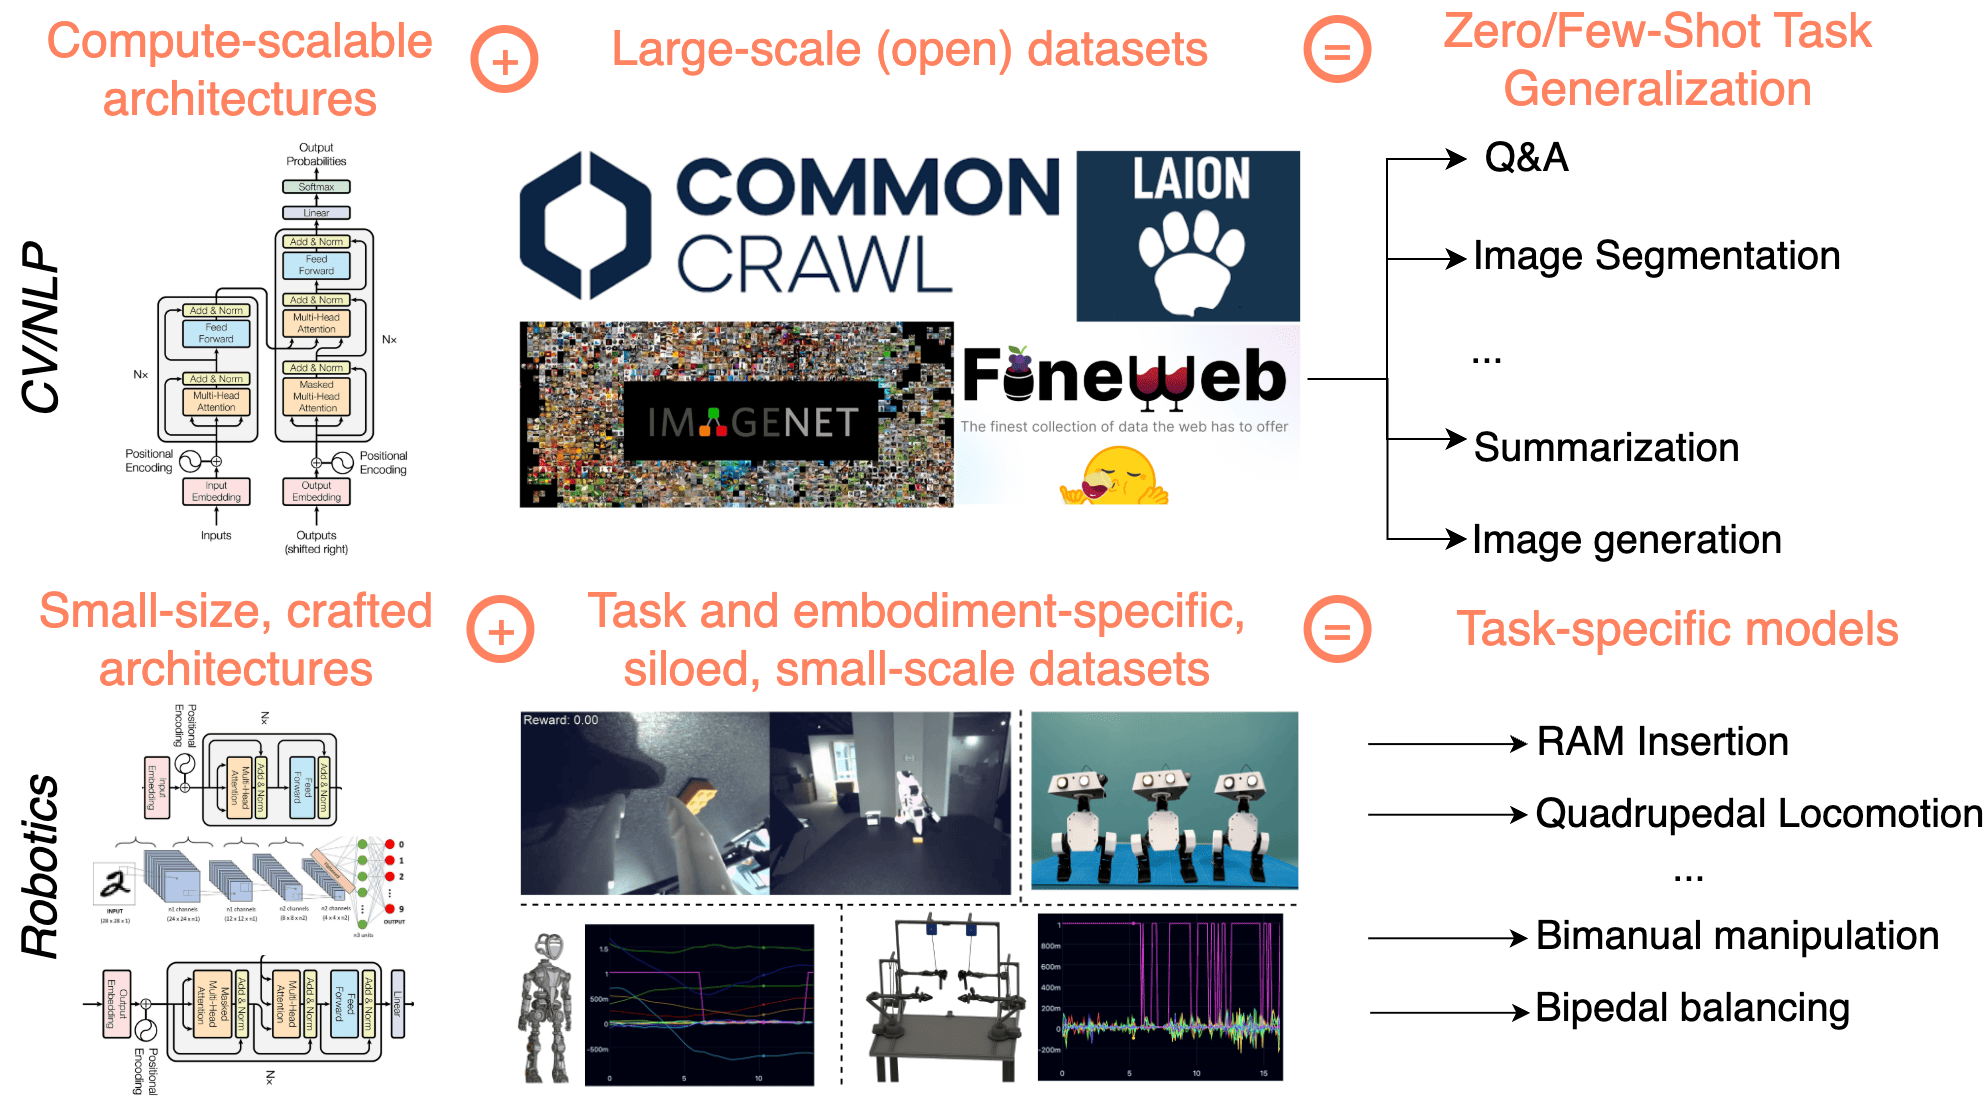
\includegraphics[width=0.9\textwidth]{figures/ch5/ch5-ml-vs-robotics-foundation.png}
    \caption{Fields within ML such as Computer Vision and NLP converged on the development of foundation models, trained on a variety of large scale models and capable to perform multiple downstream tasks (top). Conversely, robotics suffered from limited standardization in terms of the architectures used, and siloed, task specific datasets, incurring in a high degree of fragmentation which traditionally hindered the development of generalist models for robotics in favour of task-specific models (bottom).}
    \label{fig:ch5-ml-vs-robotics-foundation}
\end{figure}

\subsection{Preliminaries: Models and Data}
The remarkable success of foundation models in NLP and CV seems to be increasingly predicated on two core principles: architectural innovation and (joint) data-compute scaling.
Indeed, the transformer architecture proved very effective in capturing long-range dependencies in a variety of data formats, and its stability and expressivity made it the \emph{de facto} standard for modern large-scale models trained on internet-scale datasets.
However, in stark contrast with large-scale NLP and CV datasets~\citep{raffelExploringLimitsTransfer2023,ImageNet_VSS09}, robotics has historically developed around small, task-specific datasets. 
In turn, this traditionally hindered scalability across problems as well as results, posing concrete challenges to developing general-purpose robot learning algorithms.
Indeed, differently from the wealth of relatively readily-available task-agnostic text and images datasets on the internet, robotics data is \emph{intrinsically embodied} and thus task-specific: datasets collected for \emph{manipulation} differ significantly from \emph{locomotion}.
In particular, since each expert trajectory is tied to a specific robot platform and the operating conditions of its environment and task, data heterogeneity has long posed a \emph{methodological} challenge for scaling robotics datasets via aggregation.
Further, datasets consisting of expert demonstrations are (1) intrinsically more expensive to collect and (2) notoriously heterogeneous---different human experts may perform the same task in very different.
Beyond this, heterogeneity also raises \emph{conceptual} issues: naively mixing data across embodiments can induce negative transfer, as control strategies developed in isolation for different robot systems in different environments may even conflict when combined.
Thus, the high degree of fragmentation of robotics datasets and tasks has traditionally led to the development of \emph{specialist} policies, trained on small, task-specific datasets, developed to perform well at their designated task but that fail to generalize to new deployment scenarios (Figure~\ref{fig:ch5-ml-vs-robotics-foundation}).

\begin{figure}
    \centering
    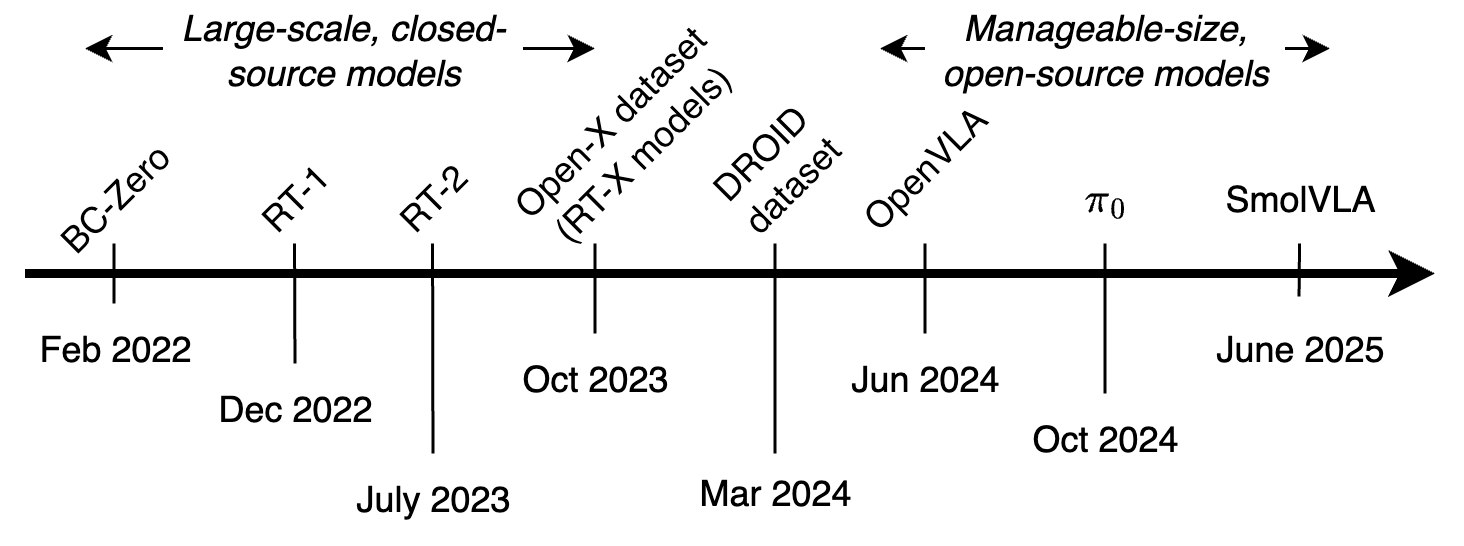
\includegraphics[width=0.8\textwidth]{figures/ch5/ch5-generalist-policies-timeline.png}
    \caption{Early efforts in the development of generalist models for robotics include BC-Zero~\citep{jangBCZZeroShotTask2022}, RT-1~\citep{brohanRT1RoboticsTransformer2023}, and RT-2~\citep{brohanRT2VisionLanguageActionModels2023}: large scale models trained on thousands of demonstrations. The open release of the Open-X~\citep{oneillOpenXEmbodimentRobotic2025} and DROID datasets~\citep{khazatskyDROIDLargeScaleInTheWild2025} fostered the development of open source models: OpenVLA~\citep{kimOpenVLAOpenSourceVisionLanguageAction2024}, \pizero~\citep{black$p_0$VisionLanguageActionFlow2024} and SmolVLA~\citep{shukorSmolVLAVisionLanguageActionModel2025}.}
    \label{fig:ch5-generalist-policies-timeline}
\end{figure}

Driven by the goal of developing generalist robot policies, the research community has increasingly explored how insights and techniques from other areas of ML can be integrated into robotics.
Figure~\ref{fig:ch5-generalist-policies-timeline} shows a timeline of some of the most popular contributions attempting at developing generalist policies.
Starting from BC-Zero, a latent variable model trained on 25k+ demonstrations, the field has now evolved into \( \pi_0 \), a transformer-based model trained on 10M+ demonstrations and exhibiting strong few-shot capabilities across tasks and embodiments.
In between, Robotics Transformer 1 (RT-1)~\citep{brohanRT1RoboticsTransformer2023} represented a significant step in the direction of developing a generalist robot policies over prior work including (1) BC-Zero~\citep{jangBCZZeroShotTask2022} and (2) Gato~\citep{reedGeneralistAgent2022}, in that~\citet{brohanRT1RoboticsTransformer2023} use a much larger and diverse set of training tasks compared to both BC-Zero and Gato.
In particular, RT-1 uses a transformer architecture, and is trained on as many as 130k human-recorded trajectories collected over 13 robots and over 17 months.
RT-1 learns to process a history of camera images and a natural language instruction, and feeds the resulting sequence of high-dimensional tokens to a transformer, trained using a \emph{classification loss on a discretized actions space} consisting of six different 256-bins, one for each joint of a 6-dof robotic arm.

In a follow-up work, the same group of authors propose a modified method to learn generalist models, leveraging (1) a more powerful architecture and (2) scaling up the dataset used~\citep[RT-2]{brohanRT2VisionLanguageActionModels2023}. 
In RT-2,~\citet{brohanRT2VisionLanguageActionModels2023} propose inheriting internet-scale semantic knowledge from large-scale multi-modal datasets to learn a single, \emph{unified model} for robotics control.
Such a model, termed \emph{Vision-Language-Action} (VLA) in the original RT-2 paper, effectively casts robot control as a language-modeling problem, and in particular as a Visual Question-Answering (VQ\&A) task, in which the output token space used to represent \emph{textual tokens} is shared with the \emph{8-bits tokens} used to represent the 256 (\( 2^8 \)) actuation levels of a 6-dof robot.
In their work,~\citet{brohanRT2VisionLanguageActionModels2023} propose co-fine-tuning large-scale VLMs such as PaLIX~\citep{chenPaLIXScalingMultilingual2023} or PaLM-E~\citep{driessPaLMEEmbodiedMultimodal2023} on a mix of (1) web and (2) robotics data, complementing VQ\&A training with robotics-specific signal, and learning to directly output robot actions in a shared token space for visual and language inputs.
In their work, the authors claim using large models trained on internet-scale data as backbones for VLAs allows models to tap into the rich semantic knowledge embedded in the VLM's parameters, interpreting instructions and unseen objects by connecting them to concepts acquired while pre-training.
For instance,~\citet{brohanRT2VisionLanguageActionModels2023} show that while RT-2 has never been explicitly trained to repurpose tools for a \emph{hammering} task, it can still combine its semantic understanding of images, so that when asked which object between (1) a piece of paper, (2) a pair of headphones or (3) a rock may be used instead of a hammer, it correctly answers (3).

Traditionally, research efforts revolved around not only training models, but also proposing datasets for the community, a costly and time-consuming process.
Due to the aforementioned embodiment gap, the data used in research efforts in robot learning have traditionally proved rather fragmented, tailored to the specific task considered by the specific group of researchers who collected it, which ultimately hindered integration.
The Open X-Embodiment project~\citep{oneillOpenXEmbodimentRobotic2025} was a landmark collaboration effort to address data fragmentation, by curating the aggregation of 60 \emph{existing} robotics datasets from 22 different robot embodiments and 21 institutions across the world, and resulted in a total 1.4M of cross-embodiments, cross-tasks, openly-available trajectories.
Besides the contribution of an aggregate, large scale dataset,~\citet{oneillOpenXEmbodimentRobotic2025} also demonstrated significant positive transfer \emph{across tasks and embodiments}, showing that \highlight{a single model trained on multi-embodiment data can outperform specialist models} trained on their respective single-embodiment datasets.
The Distributed Robot Interaction Dataset (DROID)~\citep{khazatskyDROIDLargeScaleInTheWild2025} represents another significant step towards addressing the problem of scarse and disaggregated data in robot learning, providing a unique dataset consisting of 75k+ human demonstrations collected in realistic (\emph{in-the-wild}) manipulation settings, providing another cornerstone for building general-purpose robot policies.
Recently, foundational datasets curated through large, centralized efforts, are increasingly complemented by decentralized, community-driven contributions of robotics data.
Software libraries like \lerobot~have been instrumental in enabling decentralized collection of large amounts of data, providing the infrastructure for researchers and practitioners to easily contribute trajectories from a wide range of embodiments, democratizing data access via distributed collection.

Despite these advancements, the success of large, proprietary models like RT-1 and RT-2, highlighted a growing accessibility gap in robotics research, as training and deploying large-scale robotics foundation models requires computational resources simply unattainable for most research institutions. 
The OpenVLA project~\citep{kimOpenVLAOpenSourceVisionLanguageAction2024} emerged in direct contrast to traditionally closed-source efforts to develop VLAs.
In particular,~\citet{kimOpenVLAOpenSourceVisionLanguageAction2024} trained OpenVLA by exclusively leveraging openly available data (970k+ trajectories from the Open-X dataset), and openly shared their training recipes alongside the model weights.
Architecturally, OpenVLA integrates a pre-trained vision encoder to project visual tokens into the embedding space of the Llama2-7B~\citep{touvronLlama2Open2023} language-model backbone.
The language model backbone is then used to predict \emph{discrete action tokens} over 256 activation levels.

\begin{figure}
    \centering
    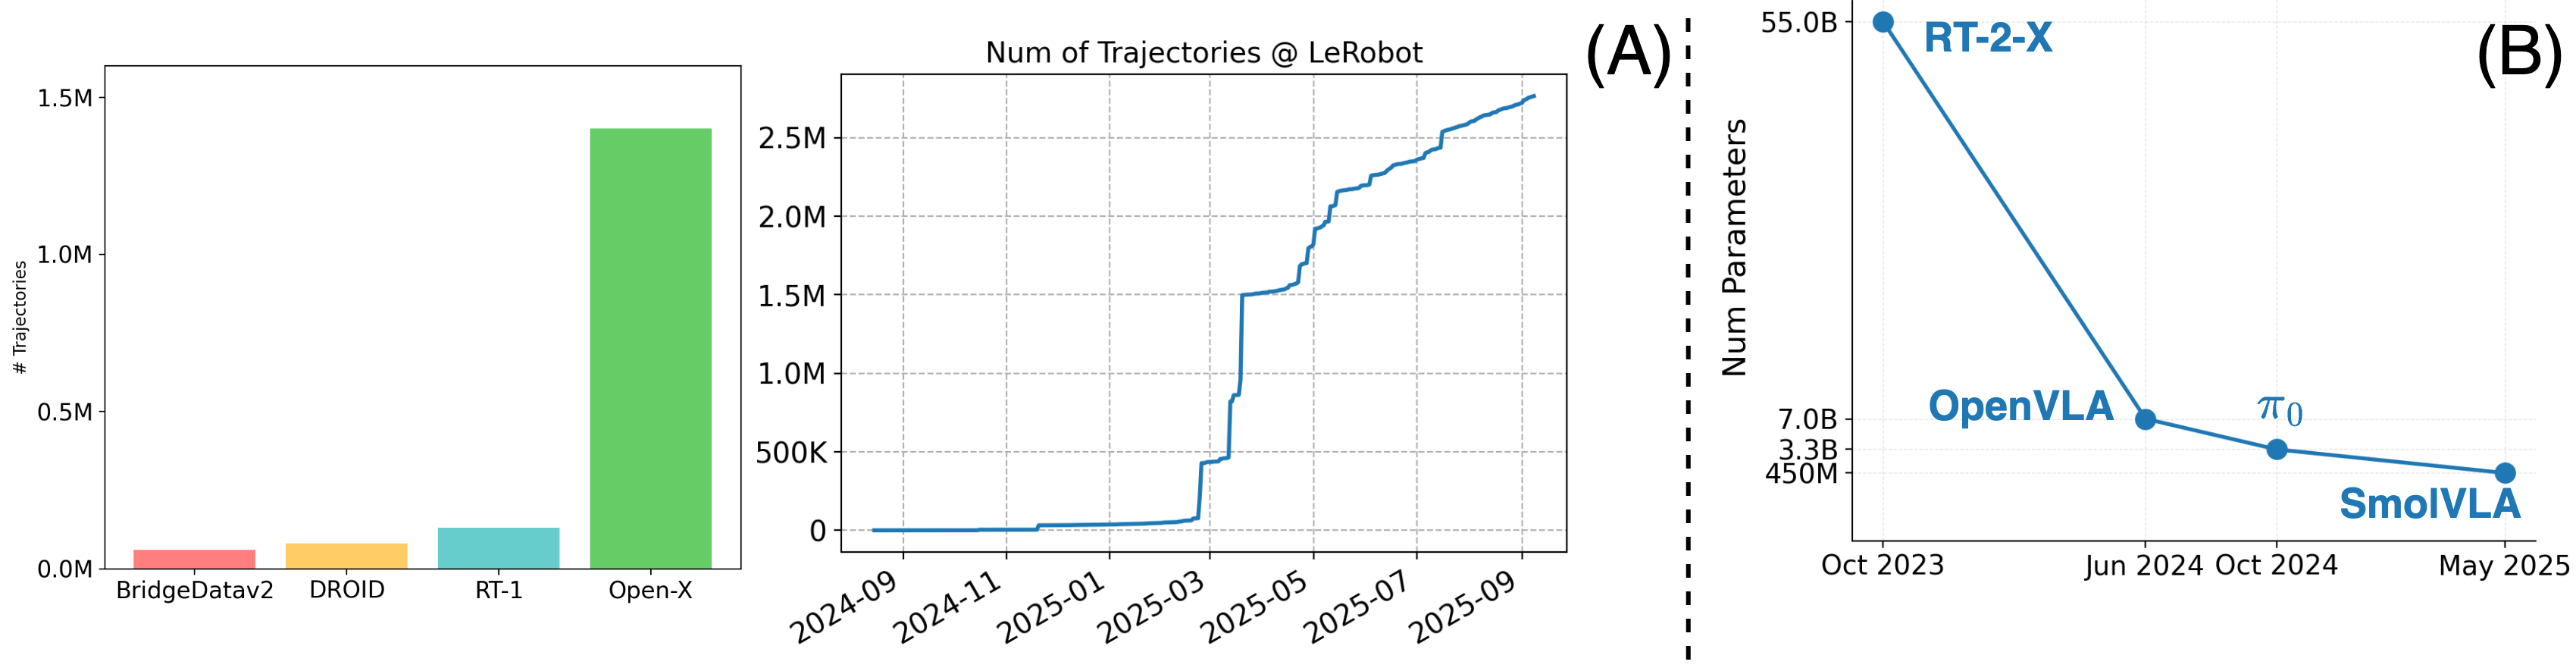
\includegraphics[width=0.9\textwidth]{figures/ch5/ch5-trends.png}
    \caption{Robot learning is undergoing a paradigmatic shift: centralized data collections (A, left) are increasingly larger, often comprising millions of demonstrations, while (A, right) decentralized data collection efforts are becoming an alternative for large scale data collection. (B) Generalist models are also becoming increasingly smaller and easier to run on limited hardware.}
    \label{fig:ch5-trends}
\end{figure}

Figure~\ref{fig:ch5-trends} shows the current trends in robot learning in terms of size and nature of the robotics datasets contributed, together with the size and accessibility of the available models.
As datasets collected via centralized, cross-institutions cooperation of increasing size are made available for the research community, decentralized datasets collected by individual researchers and practitioners also gained traction, closing the gap with academic benchmarks thanks to community-contributed datasets.
Further, models used across tasks and embodiments are increasingly becoming much more compute-efficient, and as a result the models' size has been consistently reducing over time, with consequent gains for autonomous robots in real-world, resource-constrained environments.

\subsection{VLAs}
Modern recipes to train large scale VLAs extend early efforts to learn foundation models from large amounts of data via BC, introducing significant advancements concerning both architectural and procedural aspects.
From an architectural perspective, modern VLAs such as \pizero~\citep{black$p_0$VisionLanguageActionFlow2024} leverage a \emph{unified transformer model} for efficiency of computation, while maintaining specialized sub-components within the model for visual perception and action prediction, enabling cross-task performance via language conditioning.
Crucially, modern VLAs including\pizero~\citep{black$p_0$VisionLanguageActionFlow2024} and SmolVLA~\citep{shukorSmolVLAVisionLanguageActionModel2025} adopt \emph{unified} transformer models employing disjoint set of weights (\emph{experts}) for both compute-efficient visual-semantic understanding as well as control.
Procedurally, VLAs complement advanced Vision-Language Model (VLM) backbones with action-specific modules (1) adopting mid-sized \emph{action experts} to model continuous actions distributions \( p (a_{t:t+H_a} \vert o_t) \)---avoiding discrete action tokens entirely---and (2) relying on~\emph{action chunking}~\citep[Section~\ref{sec:learning-imitation}]{zhaoLearningFineGrainedBimanual2023} as a strategy to reduce error compounding when predicting multiple actions learning from inherently non-i.i.d. data, such as demonstration data.

These architectural and procedural innovations present three benefits over task-specific methods. 
First, developing architectures that exploit internet-scale pre-trained backbones allows to fully capitalize on the vast world knowledge and skills state-of-the-art VLMs exhibit, preventig models from needing to learn visual, linguistic and semantic concepts from scratch.
Second, using generative models for continuous action distributions allows to learn rich, multimodal data distributions, a much more likely scenario in the big-data regime which is typically tackled while developing generalist policies.
Further, introducing separate components for perception and action planning enable using Mixture of Experts (MoE) architectures~\citep{fedusReviewSparseExpert2022}, which are often more efficient to run---a key feature for models deployed in real-world scenarios.
This new paradigm has been at the core of some of the most capable generalist policies developed to date, capable to few-shot adapt to novel tasks and to perform highly dexterous manipulation tasks ranging from end-to-end folding laundry to bussing tables~\citep{black$p_0$VisionLanguageActionFlow2024}.

\subsubsection{VLMs for VLAs}
VLMs are designed to handle both visual and textual modalities, most commonly by taking both images and text as inputs, generating text conditioned on the visual context.
Recent advances in VLMs have been driven by the success of LLMs, with many approaches building upon pretrained LLMs and adopting similar training paradigms to the ones used in language modeling.
Typically, VLMs~\citep{alayracFlamingoVisualLanguage2022,laurenconWhatMattersWhen2024,linVILAPretrainingVisual2024} are constructed by integrating a pretrained vision encoder~\citep{radfordLearningTransferableVisual2021,zhaiSigmoidLossLanguage2023,finiMultimodalAutoregressivePretraining2024} with a pretrained LLM~\citep{grattafioriLlama3Herd2024,jiangMistral7B2023}.
Training then proceeds in multiple multimodal stages, beginning with a large-scale pretraining on datasets containing image-text pairs~\citep{LAION-COCO,kakaobrain2022coyo700m} and interleaved vision-language corpora~\citep{OBELICS,MMC4}, all followed by a supervised fine-tuning stage on instruction-tuning datasets~\citep{LLaVA-1.5,tong2024cambrian,laurenconWhatMattersWhen2024}.
The inherent multimodal nature of VLMs enables them to jointly reason over vision and language. 
Pre-training on vast internet-scale datasets allows these models to associate visual patterns with textual descriptions, thereby acquiring a rich semantic understanding of the world---knowledge about objects, their properties, and relationships---without explicit supervision for each concept. 
In turn, integrating VLMs as the perceptual backbone for VLAs allows the latter to inherit rich, contextual world knowledge from the VLM, sidestepping the need to re-learn visual and semantic representations.
In principle, this also allows the robot to ground high-level natural language instructions in its visual context, and possibly recognize objects by connecting them to the pre-trained concepts absorbed during pre-training, improving on the possibility to generalize to novel scenarios.

Recently, compute efficiency has also become a central focus in multi-modal research. 
Several works aim to reduce training costs by using smaller, more diverse datasets~\citep{LLaVA-1.5,InstructBLIP,bai2025qwen25vl,zhu2024minigpt,tong2024cambrian}, training smaller-scale models~\citep{marafiotiSmolVLMRedefiningSmall2025, moondream,minicmpv2024}, or by adapting pretrained unimodal models by tuning only a small subset of parameters~\citep{shukor2023epalm,vallaeys2024improveddepalm,MAPL,FROMAGe,tsimpoukelli2021multimodalfrozen,BLIP-2}.
While the majority of VLM research focuses on image and text modalities, recent work has also demonstrated that similar techniques can be extended to integrate additional modalities, such as video and audio~\citep{wang2025internvideo2,liu2024kangaroo,zhang2025videollama,kong2024audioflam}---a particularly promising direction of research for robotics applications, where multiple sensor modalities can be integrated effectively. 
This trend towards efficiency is paramount for robotics applications, where policies must operate under the stringent constraints of real-world deployment. 

\subsection{\( \pi_0 \)}

\pizero~\citep{black$p_0$VisionLanguageActionFlow2024} introduce a VLA consisting of a MoE architecture consisting of (1) a pre-trained VLM backbone (Gemma 2.6B~\citep{teamGemma2Improving2024}) and (2) a dedicated action expert used to generate continuous actions via flow matching.
Images and language are embedded with PaliGemma, a VLM merging independently encoded visual and textual features deep in the network (\emph{late-fusion}), while proprioceptive state and actions chunks are routed to a smaller \emph{action expert}, initialized from scratch.
The two separate experts communicate via self-attention layers, but maintain disjoint weights to obtain query, key and values matrices at each layer, maintaining specialization while efficiently allocating computation.

\begin{figure}
    \centering
    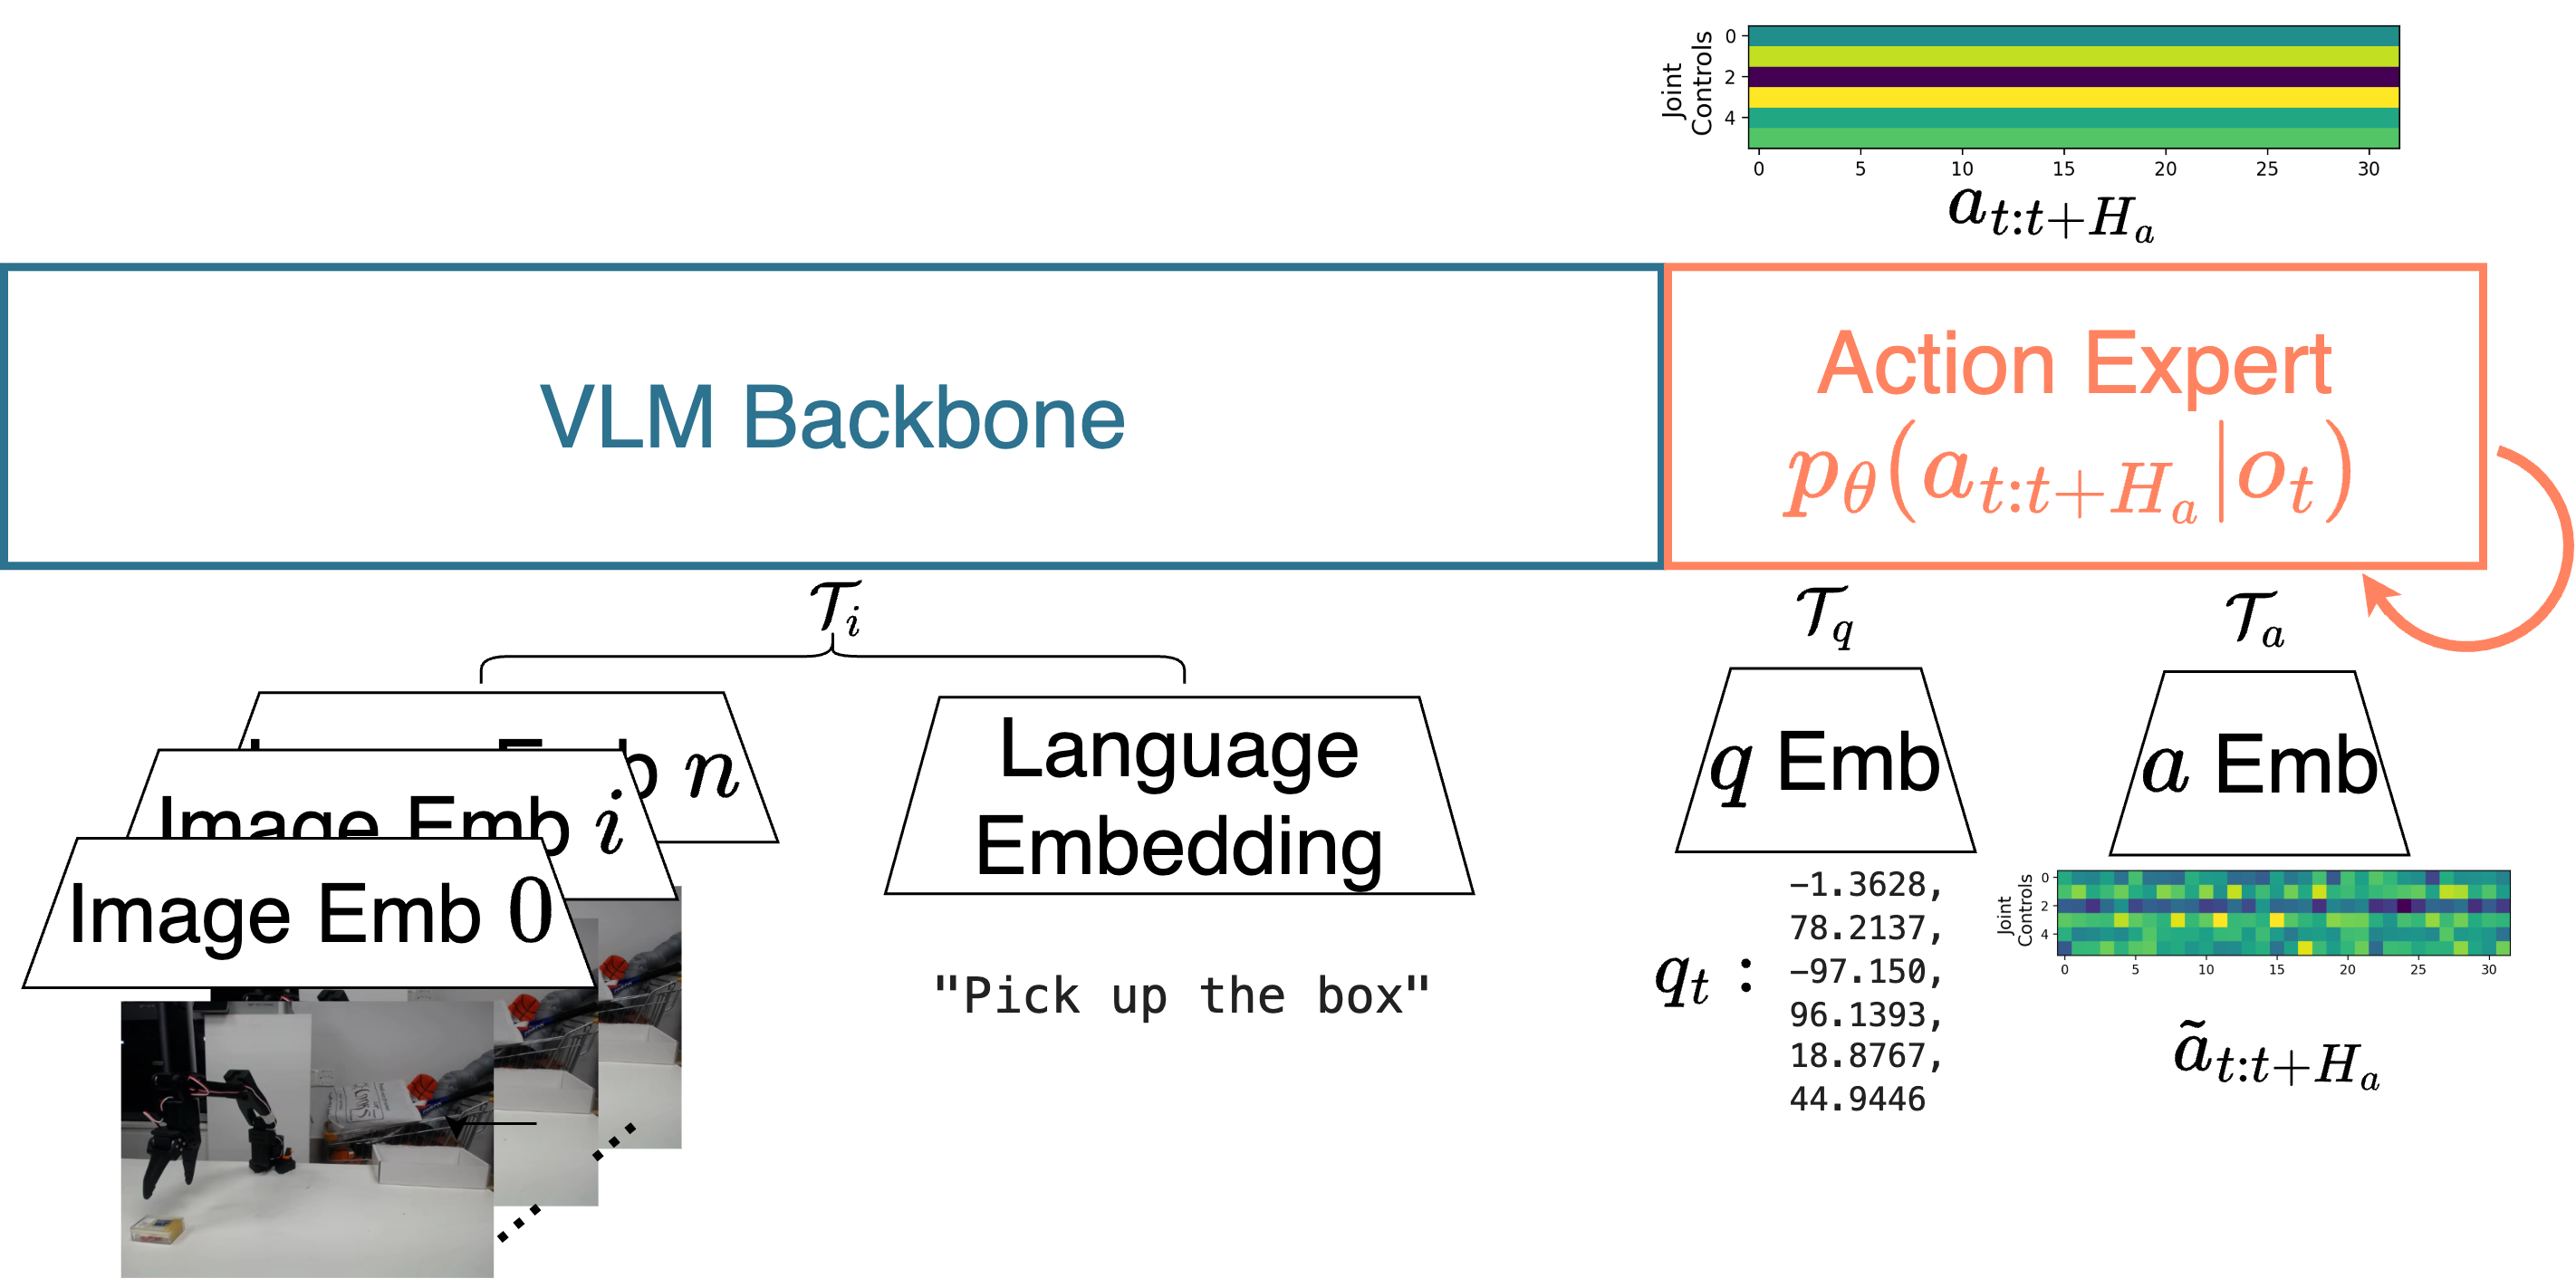
\includegraphics[width=0.9\textwidth]{figures/ch5/ch5-pi0.png}
    \caption{The \pizero~architecture, as in~\citet{black$p_0$VisionLanguageActionFlow2024}. Vision and language tokens are routed to a VLM backbone which is prevented from attending robot proprioperceptive states and action tokens, which are instead routed to a smaller subset of weights within the architecture referred to as "action expert". The architecture is trained with Flow Matching on 10M+ trajectories from a mixture of closed and openly available datasets.}
    \label{fig:ch5-pi0}
\end{figure}

Concretely, \( \pi_0 \) is a single, unified transformer with two disjoint sets of weights \( \phi, \theta\). 
A larger VLM backbone \( f_\phi \) initialized from Gemma 2.6B processes multiple image frames obtained from multiple cameras points \( [\{ I_t \}_{t=1}^n] \), as well as a language instruction \([\ell_t]\) used to describe the task considered.
Concurrently, a 300M-parameter \emph{action expert} based on a similar transformer architecture is used to process both the robot proprioperceptive state \(q_t\) and an action chunk \(a_{t:t+H_a}\) (Figure~\ref{fig:ch5-pi0}).
The different expert networks operate separately in processing the respective inputs and turn them into query, key and value matrices, and only share information between each other via self-attention layers.
The outputs from the VLM backbone are disregarded, while the vector field regressed by the action expert is used to iteratively refine the action process.
In particular, \pizero~uses a \emph{blockwise causal attention mask} over tokens belonging to three separate blocks: (1) image and language tokens \(\mathcal T_i \)  obtained from \([\{ I_t \}_{t=1}^n, \ell_t]\), (2) proprioperceptive tokens \(\mathcal T_q \) obtained from \(q_t\), and (3) the action tokens \( \mathcal T_a \) for items in the chunk \(a^{\tau}_{t:t+H_a}\) at time \( \tau \) in the flow-matching process.
Notably, \emph{within} each block the attention operations are bidirectional, while \emph{across} blocks, future blocks are masked out.
Formally, this corresponds to using an attention mask like:
\begin{equation*}
    \mathbf{A} =
    \bordermatrix{
              & \mathcal{T}_i & \mathcal{T}_q & \mathcal{T}_a \cr
    \mathcal{T}_i & \mathbf{1} & \mathbf{0} & \mathbf{0} \cr
    \mathcal{T}_q & \mathbf{1} & \mathbf{1} & \mathbf{0} \cr
    \mathcal{T}_a & \mathbf{1} & \mathbf{1} & \mathbf{1} \cr
    },
    \quad \mathbf{1}: \text{Bidirectional Attention}, \ \mathbf{0}: \text{Masked Attention} 
\end{equation*}
Note how \emph{intra}-block directional attention allows tokens to communicate freely, while \emph{inter}-block communication is mediated by the attention mask \(\mathbf{A} \).
\emph{Blockwise causal masking} effectively prevents the pre-trained perception-language tokens from attending to robotics-tokens, likely out of distribution for VLM backbones traditionally trained on large corpora of internet, non-robotics, data.
Crucially, because communication is obstructed between image-language tokens, proprioperceptive tokens and action tokens, one can cache keys and values across denoising steps at runtime time, incuring in a reduced computational footprint and faster inference.

In \pizero, both the VLM backbone and action expert are update using a \emph{flow matching} loss, and in particular are updated minimizing:
\begin{align}
    \mathcal{L}(\phi, \theta) &= 
    \mathbb{E}_{\tau, \epsilon, o_t, a_{t:t+H_a}}\Big[
        \big\Vert 
            v_\theta(\underbrace{\tau a_{t:t+H_a} + (1-\tau) \epsilon}_{\tilde a_{t:t+H_a}},\, o_t,\, \tau)
            - (\epsilon - a_{t:t+H_a})
        \big\Vert^2
    \Big], \label{eq:pi0-loss} \\
    &\tau \sim \mathrm{Beta}_{[0,s]}(1.5,1), \quad
    \epsilon \sim \mathcal{N}(\mathbf{0}, \mathbf{I}), \quad
    o_t, a_{t:t+H_a} \sim \mathcal D \notag
\end{align}
where the two experts parametrized by the separate weights \( \phi, \theta \) interact with each other via self-attention layers only, so that the action expert \( v_\theta \) internal computations also depend on the VLM backbone's parameters \( \phi \).
Importantly,~\citet{black$p_0$VisionLanguageActionFlow2024} minimize eq.~\ref{eq:pi0-loss} over both the multimodal backbone and action expert parameters, thus updating both the internal representations of the VLM and action-expert weights using BC-specific gradients.
In contrast,~\citet{driessKnowledgeInsulatingVisionLanguageAction2025} later show that failing to insulate the VLM knowledge from the flow matching gradients actually harms performance.

At runtime, inference is performed iteratively refining action chunks while numerically forward-integrating the vector field predicted by the action expert,
\begin{equation}
    a_{t:t+H_a}^{\tau + \delta} = a_{t:t+H_a}^{\tau } + \delta v_\theta(a_{t:t+H_a}^{\tau }, o_t)
\end{equation}

Flow matching~\citep[Section\ref{sec:ch4-flow-matching}]{lipmanFlowMatchingGenerative2023} can be seen as a continuous time, deterministic generalization of diffusion processes, and has proven effective in modeling highly complex multi-modal distributions, including those over images and video.
In turn, the application of flow matching to large-scale datasets of multiple human behaviors across tasks and embodiments appears rather consequential, particularly considering how it can enable faster inference via a limited number of denoising steps at test time---as few as 10, in \pizero.
In particular, the action expert is implemented as a conditional flow matching model.
Each action token embeds a noisy action \(a_i^{\tau} \in a^\tau_{t:t+H_a}\), alongside a sinusoidal encoding of the \emph{flow process} timestep \(\tau\).
The action expert then leverages full bidirectional attention across the \(H_a\) action tokens provided, and also attends to previous proprioperceptive and image-language tokens.
Interestingly, differently from a standard flow matching pipeline~\citep{lipmanFlowMatchingGenerative2023}, \(\tau\) is \emph{not} sampled from a uniform distribution \(\tau \sim \mathcal U([0,1]) \), but rather obtained from \(\tau \sim \textrm{Beta}(1.5,1) \) defined on the \( [0,s], s<1 \) support (Figure~\ref{fig:ch5-pi0-sampling-timesteps}).

\begin{wrapfigure}{r}{0.4\textwidth}
    \vspace{-10pt}
    \centering
    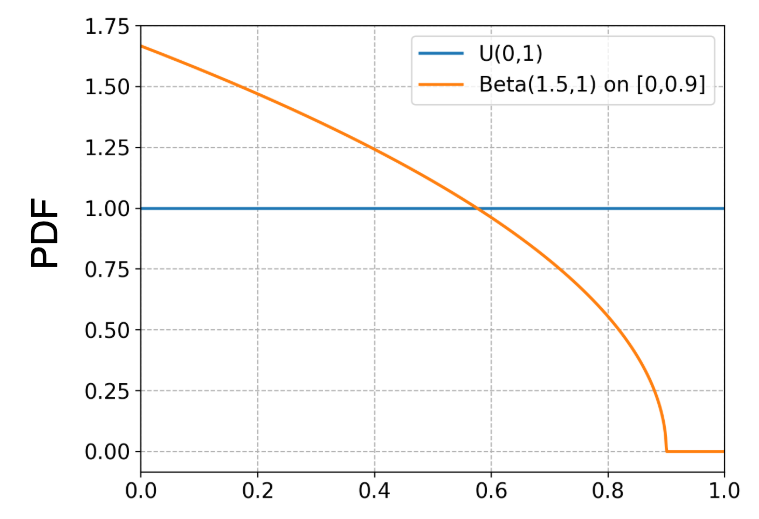
\includegraphics[width=\linewidth]{figures/ch5/ch5-pi0-sampling-timesteps.png}
    \caption{Unlike more traditional flow-matching algorithms, \pizero~uses a modified distribution to sample the timestep \( \tau \) from during training and inference, favouring earlier timestamps corresponding to noisier chunks.}
    \label{fig:ch5-pi0-sampling-timesteps}
\end{wrapfigure}

Using such Beta distribution emphasizes higher noise levels during training, a choice~\citet{black$p_0$VisionLanguageActionFlow2024} argue allows \pizero~to focus on learning to reconstruct the mean of the data distribution \( \mathbb E[a_{t:t+H_a} \vert o_t] \) over an identity map during training, in keeping with~\citet{esserScalingRectifiedFlow2024}.
To further optimize performance and reduce inference time,~\citet{black$p_0$VisionLanguageActionFlow2024} propose reducing the support of the timestep distribution to \([0,s], \ s < 1 \), as for any forward-integration step size \( \delta = 1-s \) timesteps above \(s \) are never sampled at inference time.

Besides adopting a MoE architecture with a VLM backbone initialized from a pre-trained model and trained jointly with an action expert via flow matching, \pizero~also relies on a unique pre-training corpus comprising of a mix of proprietary and open data totaling 10M+ trajectories, which in their work~\citet{black$p_0$VisionLanguageActionFlow2024} claim to be the largest dataset used to develop a foundational robotics model to date.
The dataset used to train \pizero---referred to as "the \( \pi \) dataset"---comprises a private, undisclosed portion obtained via expert teleoperation as well as openly available datasets including Open-X and DROID, with only \(\approx 9.1\%\) of the \( \pi \) being openly available.
In the \( \pi \) dataset, open datasets such as DROID and Open-X are complemeneted with expert trajectories consisting of dexterous demonstrations tasks spanning 7 robot configurations and 68 different tasks.
Crucially, \citet{black$p_0$VisionLanguageActionFlow2024} show that pre-training on the \( \pi \) dataset yields a broadly capable base model, which can be adapted via fine-tuning on narrower, higher-quality task data, which induces a fluent multi-stage behavior while retaining robustness.
In particular,~\citet{black$p_0$VisionLanguageActionFlow2024} report that, across a variety of benchmarks, the version of \pizero~pretrained on the \( \pi \) dataset and fine-tuned on extra high-quality data demonstrations \emph{consistently outperforms} a \( \pi_0^{\text{scratch}} \)~baseline trained entirely from scratch for a given specific task, which further underscores the relevance of pretraining on the \( \pi \) dataset.
\citet{black$p_0$VisionLanguageActionFlow2024} do also offer an intuition behind this finding: high-quality demonstrations of a given task tend to omit failure data, which inherently prevents an autonomous agent to learn how to recover from near-failure states.
In turn, robot trained on high-quality data exclusively with BC may as well be entirely incapable to recover from failure.
Conversely, large scale collections of human demonstrations are typically much more diverse (if anything, for their sheer scale), and typically contain rich and diverse information, which may prove suboptimal for any given task when considered in isolation but which proves invaluable in coupling with a small, narrower set of demonstrations.

Lastly,~\citet{black$p_0$VisionLanguageActionFlow2024} present cross-embodiment experiments where they demonstrate \pizero's ability to control both mobile and static manipulator robots with varying arm embodiments.
The emergence of cross-embodiment capabilities is largely to be attributed to the presence of large scale cross-embodiment data in \( \pi \) data mixture, which is in practice handled by \pizero~outputting actions with maximal configuration size across the whole \( \pi \) dataset, and zero-padding robots with fewer dofs.
\pizero~does also rely on exactly three camera views at both training and test time, and uses masked image slots for training and deployment scenarios with fewer cameras.

\subsubsection{Code Example: Using \pizero}
\begin{pbox}[label={ex:using-pizero}]{Using \pizero}
    \inputminted{python}{snippets/ch5/01_using_pi0.py}
\end{pbox}

\subsection{SmolVLA}
With VLAs in the early stage of development compared to more mature LLMs and VLMs, much of the progress made on VLAs remains proprietary, with many releases exclusively sharing the weights while withholding the data used, full experimental details and essential methodological components of training.
In constrast with this closed approach, SmolVLA~\citep{shukorSmolVLAVisionLanguageActionModel2025} is an entirely open-source research effort, which aims at democratizing the developments of robotics foundation models by open sourcing the model alongside the data used as well as the training recipes.

\begin{figure}
    \centering
    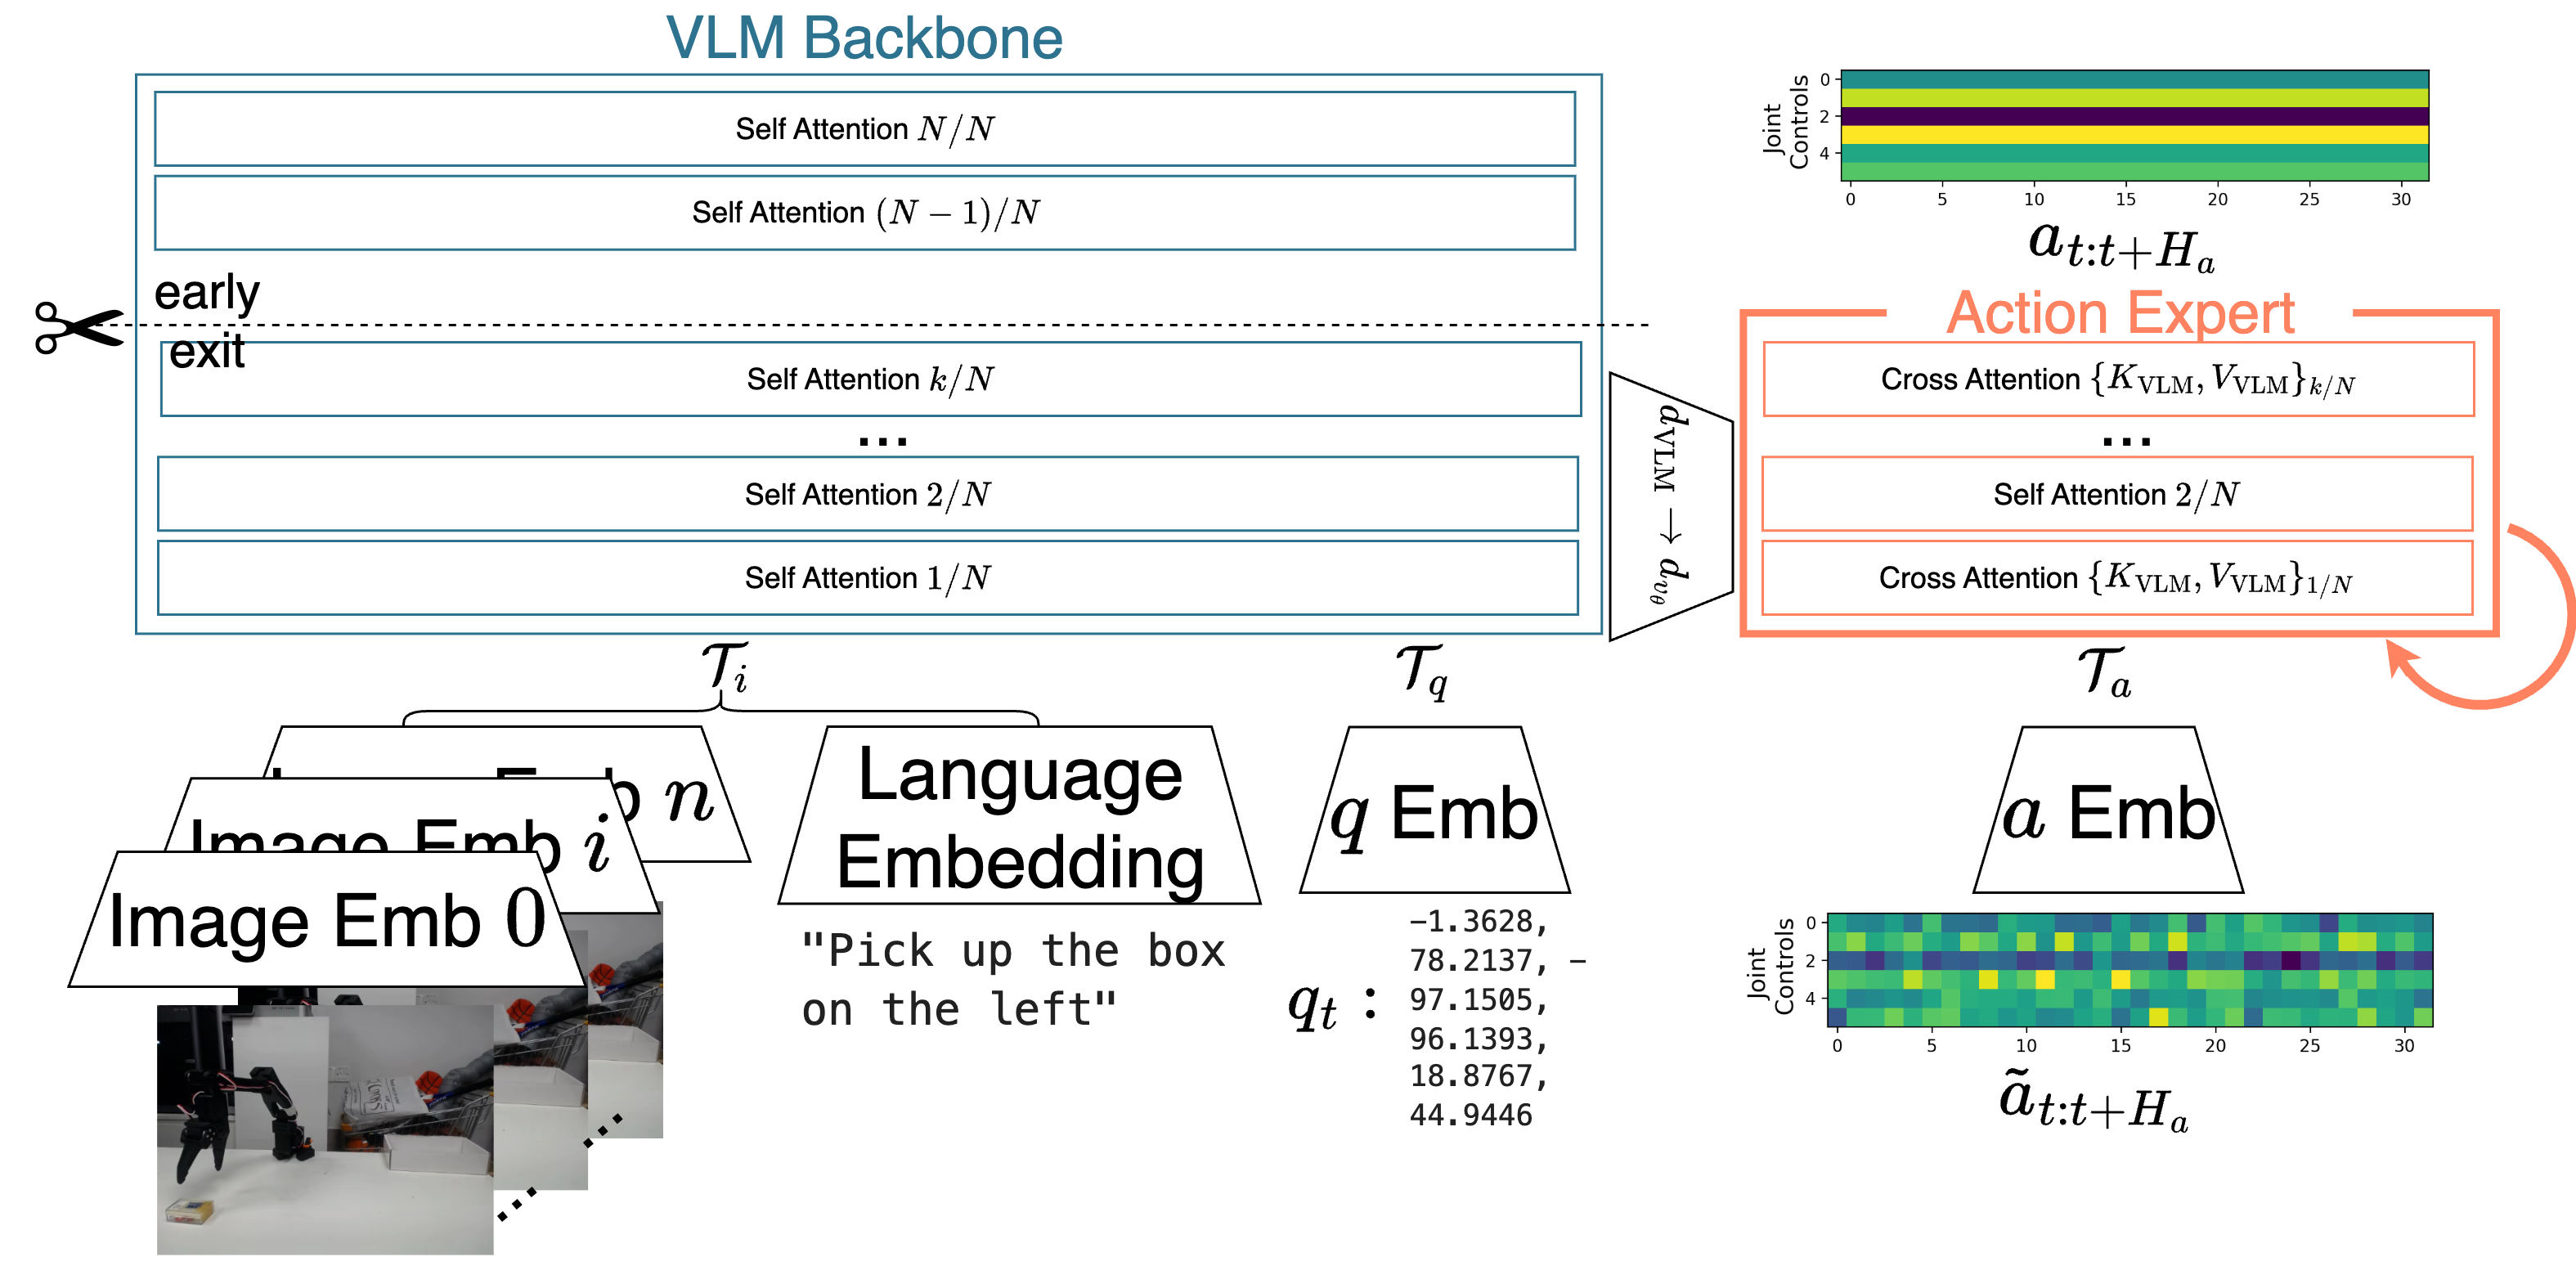
\includegraphics[width=0.9\textwidth]{figures/ch5/ch5-smolvla.png}
    \caption{The SmolVLA architecture, as in~\citet{shukorSmolVLAVisionLanguageActionModel2025}. SmolVLA is a compact MoE model trained with flow matching to denoise action chunks. Vision and language tokens are fed to a VLM backbone, and share information with the proprioperceptive and action tokens via the attention mechanism. The attention expert interleaves SA and CA layers for further conditioning on the visual features from the VLM backbone. SmolVLA skips computations and reduces the visual tokens, resulting in 7x less memory usage than \pizero~(450M parameters vs. \pizero's 3.3B).}
    \label{fig:ch5-smolvla}
\end{figure}

While encouraging efforts like \pizero~\citep{black$p_0$VisionLanguageActionFlow2024} demonstrate the feasibility of open VLA systems, they remain (1) large and compute-intensive and (2) dependent on closed datasets collected via centralized efforts on costly robotic platforms, which ultimately hinders the accessibility of the method altogether.
SmolVLA mitigates both these issues by (1) prioritizing a compact, compute-efficient VLA design and (2) targeting community-contributed datasets on accessible robotic platforms such as the SO-100 and SO-101 arms.
Similarly to \pizero, SmolVLA (Figure~\ref{fig:ch5-smolvla}) employs a MoE architecture combining a pretrained VLM backbone with a dedicated action expert, and trains with flow matching.
To ensure efficiency and accessibility, SmolVLA adopts SmolVLM-2~\citep{marafiotiSmolVLMRedefiningSmall2025} as its VLM backbone, considering SmolVLM-2's reduced size and capability to process multiple image inputs alongside text items.
SmolVLM-2 uses SigLIP~\citep{zhaiSigmoidLossLanguage2023} as vision encoder, producing visual features for a SmolLM2 language decoder~\citep{allalSmolLM2WhenSmol2025}.
Further, SmolVLA adopts a smaller action expert consisting of \(\sim\)100M parameters and an interleaved stack of self and cross-attention layers.
To improve efficiency, the action expert adopts a reduced embedding dimension compared to the VLM backbone, resulting in \( d_{v_\theta} = 0.75 d_{\text{VLM}} \).
\citet{shukorSmolVLAVisionLanguageActionModel2025}'s design choices thus result in a much smaller size model compared to \pizero, consisting of ca. 450M parameters versus \pizero's 3.3B parameters.

In practice, SmolVLA consumes multi-view RGB images, a natural-language instruction, and projected sensorimotor state token as inputs, together with the noised \emph{action chunk} \( \tilde{a}_{t:t+H_a} \) the action expert \( v_\theta \) is trained to denoise.
The robot proprioperceptive states are projected to a shared token space with the VLM to match \( d_{\text{VLM}} \), and successively projected into the expert's token space.
Similarily to \pizero, SmolVLA adopts separate experts communicating exclusively through self-attention layers, which however do not employ blockwise causal attention masking and rather favour simple causal masking.

In contrast with \pizero, the action expert interleaves \emph{cross-attention} (CA) and \emph{self-attention} (SA) layers, a choice shown to yield higher success and smoother action chunks in practice.
While in the expert SA layers tokens are used to obtain queries, keys and values, CA layers use action tokens only as queries, and instead project visual, language and proprioperceptive tokens from the VLM backbone to a shared embedding space to then obtain keys and values.
Notably, keys and values can be cached  here as well, resulting in performance gains at inference time.

SmolVLA also trims down both token and layer compute.
First, it \emph{reduces visual tokens} via pixel shuffling to a fixed budget of 64 tokens per frame, foregoing the tiling used during VLM pretraining for the sake of runtime efficiency. 
Second, it \emph{skips upper VLM layers}, as only features from the first \(N\) decoder layers, with \(N=L/2\), are consumed, which provides a good speed-performance trade-off and effectively halves compute needs for the larger part of SmolVLA.
Beyond model compactness, SmolVLA also contributes an inference stack that decouples action prediction from execution for responsiveness on modest hardware (Section~\ref{sec:ch4-async-inference}).

Departing from reliance on proprietary datasets, SmolVLA pretrains exclusively on 450+ \emph{community datasets}, totaling 20k+ trajectories. 
Because instructions in community contributed dataset can be noisy or missing, the authors re-annotate tasks with a small off-the-shelf VLM using frames sampled from the dataset, and standardize camera viewpoints by mapping sources to a consistent top/wrist/side ordering.
At test time, similarily to \pizero, SmolVLA forward-integrates flow over 10 steps, resulting in fast inference.
SmolVLA proves effective across a range of both real-world and simulated environments, rivaling \pizero~while being close to 40\% faster and consuming 6x less memory~\citep{shukorSmolVLAVisionLanguageActionModel2025}.

\subsubsection{Code Example: Using SmolVLA}
\begin{pbox}[label={ex:using-pizero}]{Using SmolVLA}
    \inputminted{python}{snippets/ch5/02_using_smolvla.py}
\end{pbox}
